Die Anomalienerkennung mit ARX als Reparaturverfahren hat den Vorteil, dass die
markierten Werte effektiv für die Reparatur ausgenutzt werden, indem der
Fehlerverlauf auf zukünftige und unmarkierte Datenpunkte berücksichtigt wird.
Wie im Kapitel \ref{sec:grundlagen} vorgestellt, führt die Anwendung von
ARX dennoch zu drastischen Veränderungen der Messungen, obwohl z.B. GPS- oder
Sensorenaufnahmen häufig auch im Fehlerfall beinahe korrekte Werte liefern.
Daher wird das Minimum-Change-Prinzip gefordert, dass Messungen nur relativ
leicht modifiziert.  Die gewünschte Vereinbarung des Erkennen von natürlichen
Fehlerverläufen in der Anomalienerkennung und das  Minimum-Change-Prinzip
bewegte die Autoren des Papers zu der Entwicklung von Iterative Minimum
Repairing (kurz IMR).  Dieses Kapitel beschäftigt sich mit den
allgemeinen Fall und zwei laufzeitbedingte Optimierungen von IMR. Ein Nachteil
von IMR ist jedoch die hohe geforderte Laufzeit - auch im Falle beider
Optimierungen -, sodass IMR als Online-Algorithmus eigentlich nicht angewandt
werden kann. Durch zusätzliche Annahmen lässt sich jedoch ein
Online-Algorithmus formulieren, dass diesen Anforderungen genügt. Die
vorgestellten Versionen des IMR werden im Kapitel \ref{sec:evaluation}
miteinander als auch mit den State-of-art Verfahren aus Kapitel
\ref{sec:grundlagen} gegenübergestellt.

\subsection{Allgemeines IMR}

Der Algorithmus IMR ist im Alg. \ref{alg:imr} hinterlegt.  Sei $y^{(k)}$ die
Reparatur in der k.ten Iteration. Initialisiert wird $y^{(0)}$ mit der Messung
x, wenn kein markierte Wert vorliegt, ansonsten wird der markierte Wert
benutzt. Während der Prozedur bleiben die markierten Werte in $y^{(k)}$
unverändert.  Grundsätzlich lässt sich eine Iteration des Algorithmus in
folgende Schritte unterteilen:
\begin{enumerate}
    \item Parameterschätzung (Zeile 4): Der Parametervektor $\phi^{(k)}$ für ARX(p) wird
bestimmt.
    \item Kandidaten für die Reparatur (Zeile 5): Nach ARX(p) werden für die unmarkierten
        Werte Vorhersagewerte $\hat{y}$ als mögliche Reparaturkandidaten ermittelt.
    \item Reparatur (Zeile 6): Ausschließlich ein Reparaturwert wird
        ausgewählt, sodass nach den Minimum-Change-Prinzip das temporäre
        Reparaturergebnis $y^{(k)}$ gering von der Messung $x$ abweicht. Die
        Abweichung des Reparaturwert muss jedoch größer als der gewählter
        Schwellenwert $\tau$ sein.
\end{enumerate}
Dabei gibt es zwei Bedingungen für die Terminierung. Entweder gab es keinen
Erfolg für die Reparatur, d.h. die Repaturergebnisse haben sich nicht
signifikant bezüglich $\tau$ geändert, so wird die letzte Reparatursequenz
ausgegeben. Die Problemstellung der Konvergenz ist für den allgemeinen Fall
jedoch nicht gezeigt. In den Experimenten, präsentiert in Kapitel
\ref{sec:evaluation}, hat IMR stets konvergiert. Aus praktischer Sicht braucht
man dennoch eine Garantie der Terminierung, weshalb eine ober Schranke der Iteration
max-num-iterations als zweite Option benötigt wird. 

\begin{algorithm}
\caption{IMR}
\label{alg:imr}
    \begin{algorithmic}[1]
\STATE \textbf{Eingabe}: Messung $x$, markierte Werte $x^{\text{truth}}$, Ordnung $p$ und Schwellenwert $\tau$
\STATE \textbf{Ausgabe}: Reparatur $y$ mit unveränderten markierten Werte 
\FOR{$k \gets 0$ \TO max-num-iterations}
\STATE {$\phi^{(k)} \gets$ Estimate$(x,y^{(k)})$}
    \STATE { $\hat{y} \gets$ Candidate$(x,y^{(k)}, phi^{(k)})$}
    \STATE { $y^{(k+1)} \gets$ Evaluate$(x,y^{(k)}, \hat{y})$}
        \IF{ Converge($y^{(k)}, y^{(k+1)}$) }
        \STATE {\textbf{break}}
        \ENDIF
 \ENDFOR
    \RETURN $y^{(k)}$
\end{algorithmic}
\end{algorithm}
~\\
\textbf{Beispiel 2} Es seien $x$, $x^{\text{truth}}$ und $x^{\text{truth}*}$ wie in Beispiel 1. Zusätzlich sei für IMR die Ordnung $p=1$ und der Schwellenwert $\tau$ gegeben.
Nach dem IMR im Alg. \ref{alg:imr} wird $y^{(0)}$ zunächst wie folgt initialisiert: 
\[
     y^{(0)} =          \{6, 5.6, 5.4, 8.3, 7.7, 5.4, 5.6, 5.9, 6.3, 6.8, 7.5, 8.5\}
\]
Durch die Parameterschätzung hat sich ein Wert von $\phi^{(1)} = 0.5$ ergeben.
Nach ARX(1) ergeben sich die Reparaturkandidaten $\hat{y}$ wie in Abb.
\ref{fig:2}.  In der Darstellung lässt sich erkennen, dass jeder
Reparaturkandidat mit der Messung $x$ außer an Stelle 4 übereinstimmt. Jene
Werte können daher nicht in die Reparatur einfliessen, da der Abstand zu der
Messung nicht größer als $\tau = 0.1$ ist. Der einzige Kandidat ist daher
$\hat{y}_4 = 6.2$, welcher dann für $y^{(1)}$ ausgewählt wird, da $|y^{(0)}_4 -
\hat{y}_4| > \tau$ ist. Gäbe es noch weitere Kandidaten mit dieser Eigenschaft,
so würde der Kandidat herangezogen werden, der an der Messung $x$ am nächsten kommt.
Aufgrund dieser Reparatur an der Stelle 4 wird in der nächsten Iteration der
Reparaturkandidat an der Stelle 5 wegen seiner Nachbarschaft zu 4 ebenfalls
beeinflusst, wohingegen die anderen unmarkierten Werte unberührt bleiben. Das
Ergebnis bis zur Konvergenz, also bis kein Reparaturkandidant größer als $\tau$
abweicht, ist in der Abb. \ref{fig:1} nachzuvollziehen.

\begin{figure}
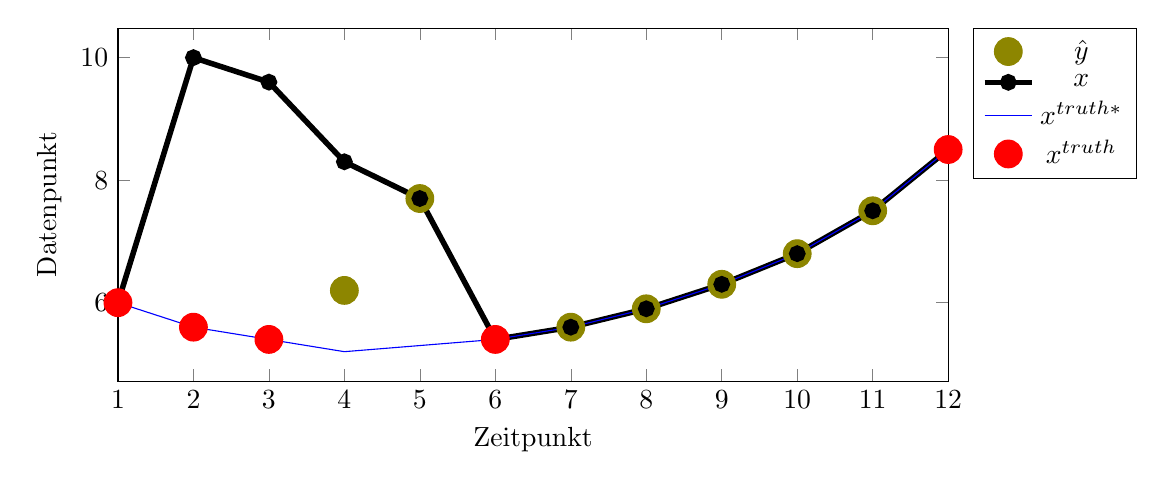
\begin{tikzpicture}
\begin{axis}[width=\textwidth,
    height=.5\textwidth,
xlabel=Zeitpunkt,
ylabel=Datenpunkt,
legend pos=outer north east,
xmin=1,
xmax=12
]
\addplot[only marks, olive,mark size=5.0pt] table{
Zeitpunkt Wert 
4 6.2
5 7.7
7 5.6
8 5.9
9 6.3
10 6.8
11 7.5
};
    \addlegendentry{$\hat{y}$}
\addplot[black, line width=2.0pt, mark size=2.0pt, mark=*]  table{
Zeitpunkt Wert 
1 6
2 10
3 9.6
4 8.3
5 7.7
6 5.4
7 5.6
8 5.9
9 6.3
10 6.8
11 7.5
12 8.5
};
 \addlegendentry{$x$}
    \addplot[blue,mark size=5.0pt] table{
Zeitpunkt Wert 
1 6
2 5.6
3 5.4
4 5.2
5 5.3
6 5.4
7 5.6
8 5.9
9 6.3
10 6.8
11 7.5
12 8.5
};
\addlegendentry{$x^{\text{truth*}}$}
\addplot[only marks, red, mark size=5.0pt] table{
Zeitpunkt Wert 
1 6
2 5.6
3 5.4
6 5.4
12 8.5
};
\addlegendentry{$x^{\text{truth}}$}
% if you have the file, you can do
% \addplot table {datafile.csv};
\end{axis}
\end{tikzpicture}
    \caption{Beispiel 2.}\label{fig:2}
\end{figure}
~\\
Wohingegen das Ermitteln der Reparaturkandidaten und die Auswahl einer dieser Reparaturkandidaten laufzeittechnisch als unproblematisch beurteilt werden kann,
ist die Laufzeit der Parameterschätzung kritisch. Wie im Kapitel \ref{sec:grundlagen} zu sehen, kann die Parameterschätzung durch die Yule-Walker Gleichung oder durch den Satz der kleinsten Quadrate approximiert gelöst werden. In IMR hat man sich dafür entschieden, den Satz der kleinsten Quadrate für das Lösen von $\phi$ anzuwenden:
\[
    \phi^{(k)} = \left(\left(Z^{(k)}\right)' Z^{(k)} \right)^{-1} \left(Z^{(k)}\right)'V^{(k)}
\]
mit
\[
    V^{(k)} = \left(\begin{matrix}
        y^{(k)}_{p+1} - x_{p+1}\\
        y^{(k)}_{p+2} - x_{p+2}\\
        \vdots\\
        y^{(k)}_{n} - x_{n}
    \end{matrix}\right),~~~~~~~
    \phi^{(k)} = \left(\begin{matrix}
        \phi_1^{(k)}\\
        \phi_2^{(k)}\\
        \vdots\\
        \phi_p^{(k)}\\
    \end{matrix}\right)
\]
~\\
~\\
\[
    Z^{(k)} = \left(\begin{matrix}
        y_{p}^{(k)} - x_{p} & y_{p-1}^{(k)} - x_{p-1} & \cdots & y_{1}^{(k)} - x_{1}\\
        y_{p+1}^{(k)} - x_{p+1} & y_{p}^{(k)} - x_{p} & \cdots & y_{2}^{(k)} - x_{2}\\
        \vdots & \vdots & \ddots & \vdots \\
        y_{n-1}^{(k)} - x_{n-1} & y_{n-2}^{(k)} - x_{n-2} & \cdots & y_{n-p}^{(k)} - x_{n-p}\\
    \end{matrix}\right)
\]
Die Notiz des Hochkommata an den Matrizen, wie z.B. $\left(Z^{(k)}\right)'$ bedeuten, dass die Matrizen transponiert sind.
\\
\\
\textbf{Beispiel 3.} Es seien alle Zeitreihen aus Beispiel 2 gegeben. Mit den
Satz der kleinsten Quadrate soll nun der Parameter $\phi$ geschätzt werden,
dass in Beispiel 2 mit $0.5$ angegeben wurde. Hieraus ergeben sich folgende Matrizen:
\begin{itemize}
    \item $ V^{(0)}= \{-4.4, -4.2, 0, 0, 0, 0, 0, 0, 0, 0, 0\}$
    \item $Z^{(0)} = \{0, -4.4, -4.2, 0, 0, 0, 0, 0, 0, 0, 0\}$
\end{itemize}
Hieraus ergibt sich folgende Schätzung:
\[
    \phi^{(0)} = \frac{-4.4 * (-4.2)}{(-4.4)^2 + (-4.2)^2} = 0.5
\]


\subsection{MP-IMR}

Um IMR von der Laufzeit zu optimieren, bietet es sich an, den Fokus auf die
Parameterschätzung zu setzen. Wie im Beipiel 3 zu vermerken, enthalten viele
Einträgen in der Matrix $V^{(0)}$ und $Z^{(0)}$ den Wert 0. Schaut man sich den
entsprechenden Aufbau beider Matrizen an, so bestehen alle Einträge aus den
Wert $y^{(k)}_i - x_i$. Da in der Praxis sehr wenig markierte Daten zur
Verfügung stehen und selbst die markierten Werte relativ nahe an der Messung
sind -- ansonsten würde man das Minimum-Change-Prinzip garnicht berücksichtigen
-- werden die Matrixen mit hoher Wahrscheinlichkeit dünnbesetzt sein. Wenn
ganze Zeilen aus 0en bestehen, so lassen sich diese auch einfach entfernen.
Diese Variante des IMR wird Matrix-Pruning-IMR (MP-IMR) genannt. Sei $z^{(k)} =
y^{(k)}_i - x_i$, dann lässt sich folgender Satz formulieren:
\begin{theorem}
    Für jede beliebige Zeile in $Z^{(k)}$, bezeichnet durch $Z^{(k)}_r$ mit $r$
    als der Zeilenindex, dessen Werte ausschließlich aus 0en besteht, d.h.
    $z^{(k)}_r+p-1 = z^{(k)}_r+p-2 = \cdots = z_r^{(k)} = 0$,  dann ist
    garantiert, dass das Löschen dieser Zeile und die zugehörige Zeile in
    $V_r^{(k)} = \left(z^{(k)}_{p+r}\right)$ in $V^{(k)}$ und $Z^{(k)}$ zu der
    selben Parameterschätzung $\phi^{(k)}$ führt.
    \label{theorem:mp}
\end{theorem}
~\\
\textbf{Beispiel 4.} Wie in Beispiel 3 soll $\phi$ abgeschätzt werden; diesmal
mit MP-IMR.  Sowohl $V^{(0)}$ und $Z^{(0)}$ haben die Größe 11 x 1. Nach Satz
\ref{theorem:mp} können die Zeilen 1 und ab Zeile 3 entfernt werden, sodass man
die reduzierten Matrizen $V^{(0)} = \{-4.2, 0\}'$ und $V^{(0)} = \{-4.2, 0\}'$
mit einer Größe von 2x1 erhält. Hieraus ergibt sich der selbe Berechnung wie in
Beispiel 3.

